\documentclass[aspectratio=169,11pt]{beamer}

\usetheme{Singapore}
\usepackage[utf8]{inputenc}
\usepackage{amsmath}
\usepackage{amsfonts}
\usepackage{amssymb}
\usepackage{graphicx}
\usepackage{hyperref}

% Setup the bibliography
\usepackage[style=authortitle,backend=bibtex]{biblatex}
\addbibresource{bibliography.bib}
\setbeamertemplate{bibliography item}[text]
\setbeamerfont{footnote}{size=\tiny}

% Allow footnotes with no number
\newcommand\blfootnote[1]{%
  \begingroup
  \renewcommand\thefootnote{}\footnote{#1}%
  \addtocounter{footnote}{-1}%
  \endgroup
}

% Allow section title slides
\AtBeginSection[]{
  \begin{frame}
  \vfill
  \centering
  \begin{beamercolorbox}[sep=8pt,center,shadow=true,rounded=true]{title}
    \usebeamerfont{title}\insertsectionhead\par%
  \end{beamercolorbox}
  \vfill
  \end{frame}
}

\author{Dr Stephen Pederson}
\title{Lecture 3: Microarray Technology}
\subtitle{BIOINF3005/7160: Transcriptomics Applications}
%\setbeamercovered{transparent} 
\setbeamertemplate{navigation symbols}{} 
\logo{
	
\includegraphics[scale=0.3]{figures/UoA_logo_col_vert.png} 
} 
\institute{Bioinformatics Hub, \\The University of Adelaide} 
\date{March 23rd, 2020} 
\subject{BIOINF3005/7160: Transcriptomics Applications} 


\begin{document}

\begin{frame}
\titlepage
\end{frame}

\begin{frame}
\footnotesize
\tableofcontents
\end{frame}



\section{Microarray Technology}

\begin{frame}{Microarrays}

	\begin{center}
	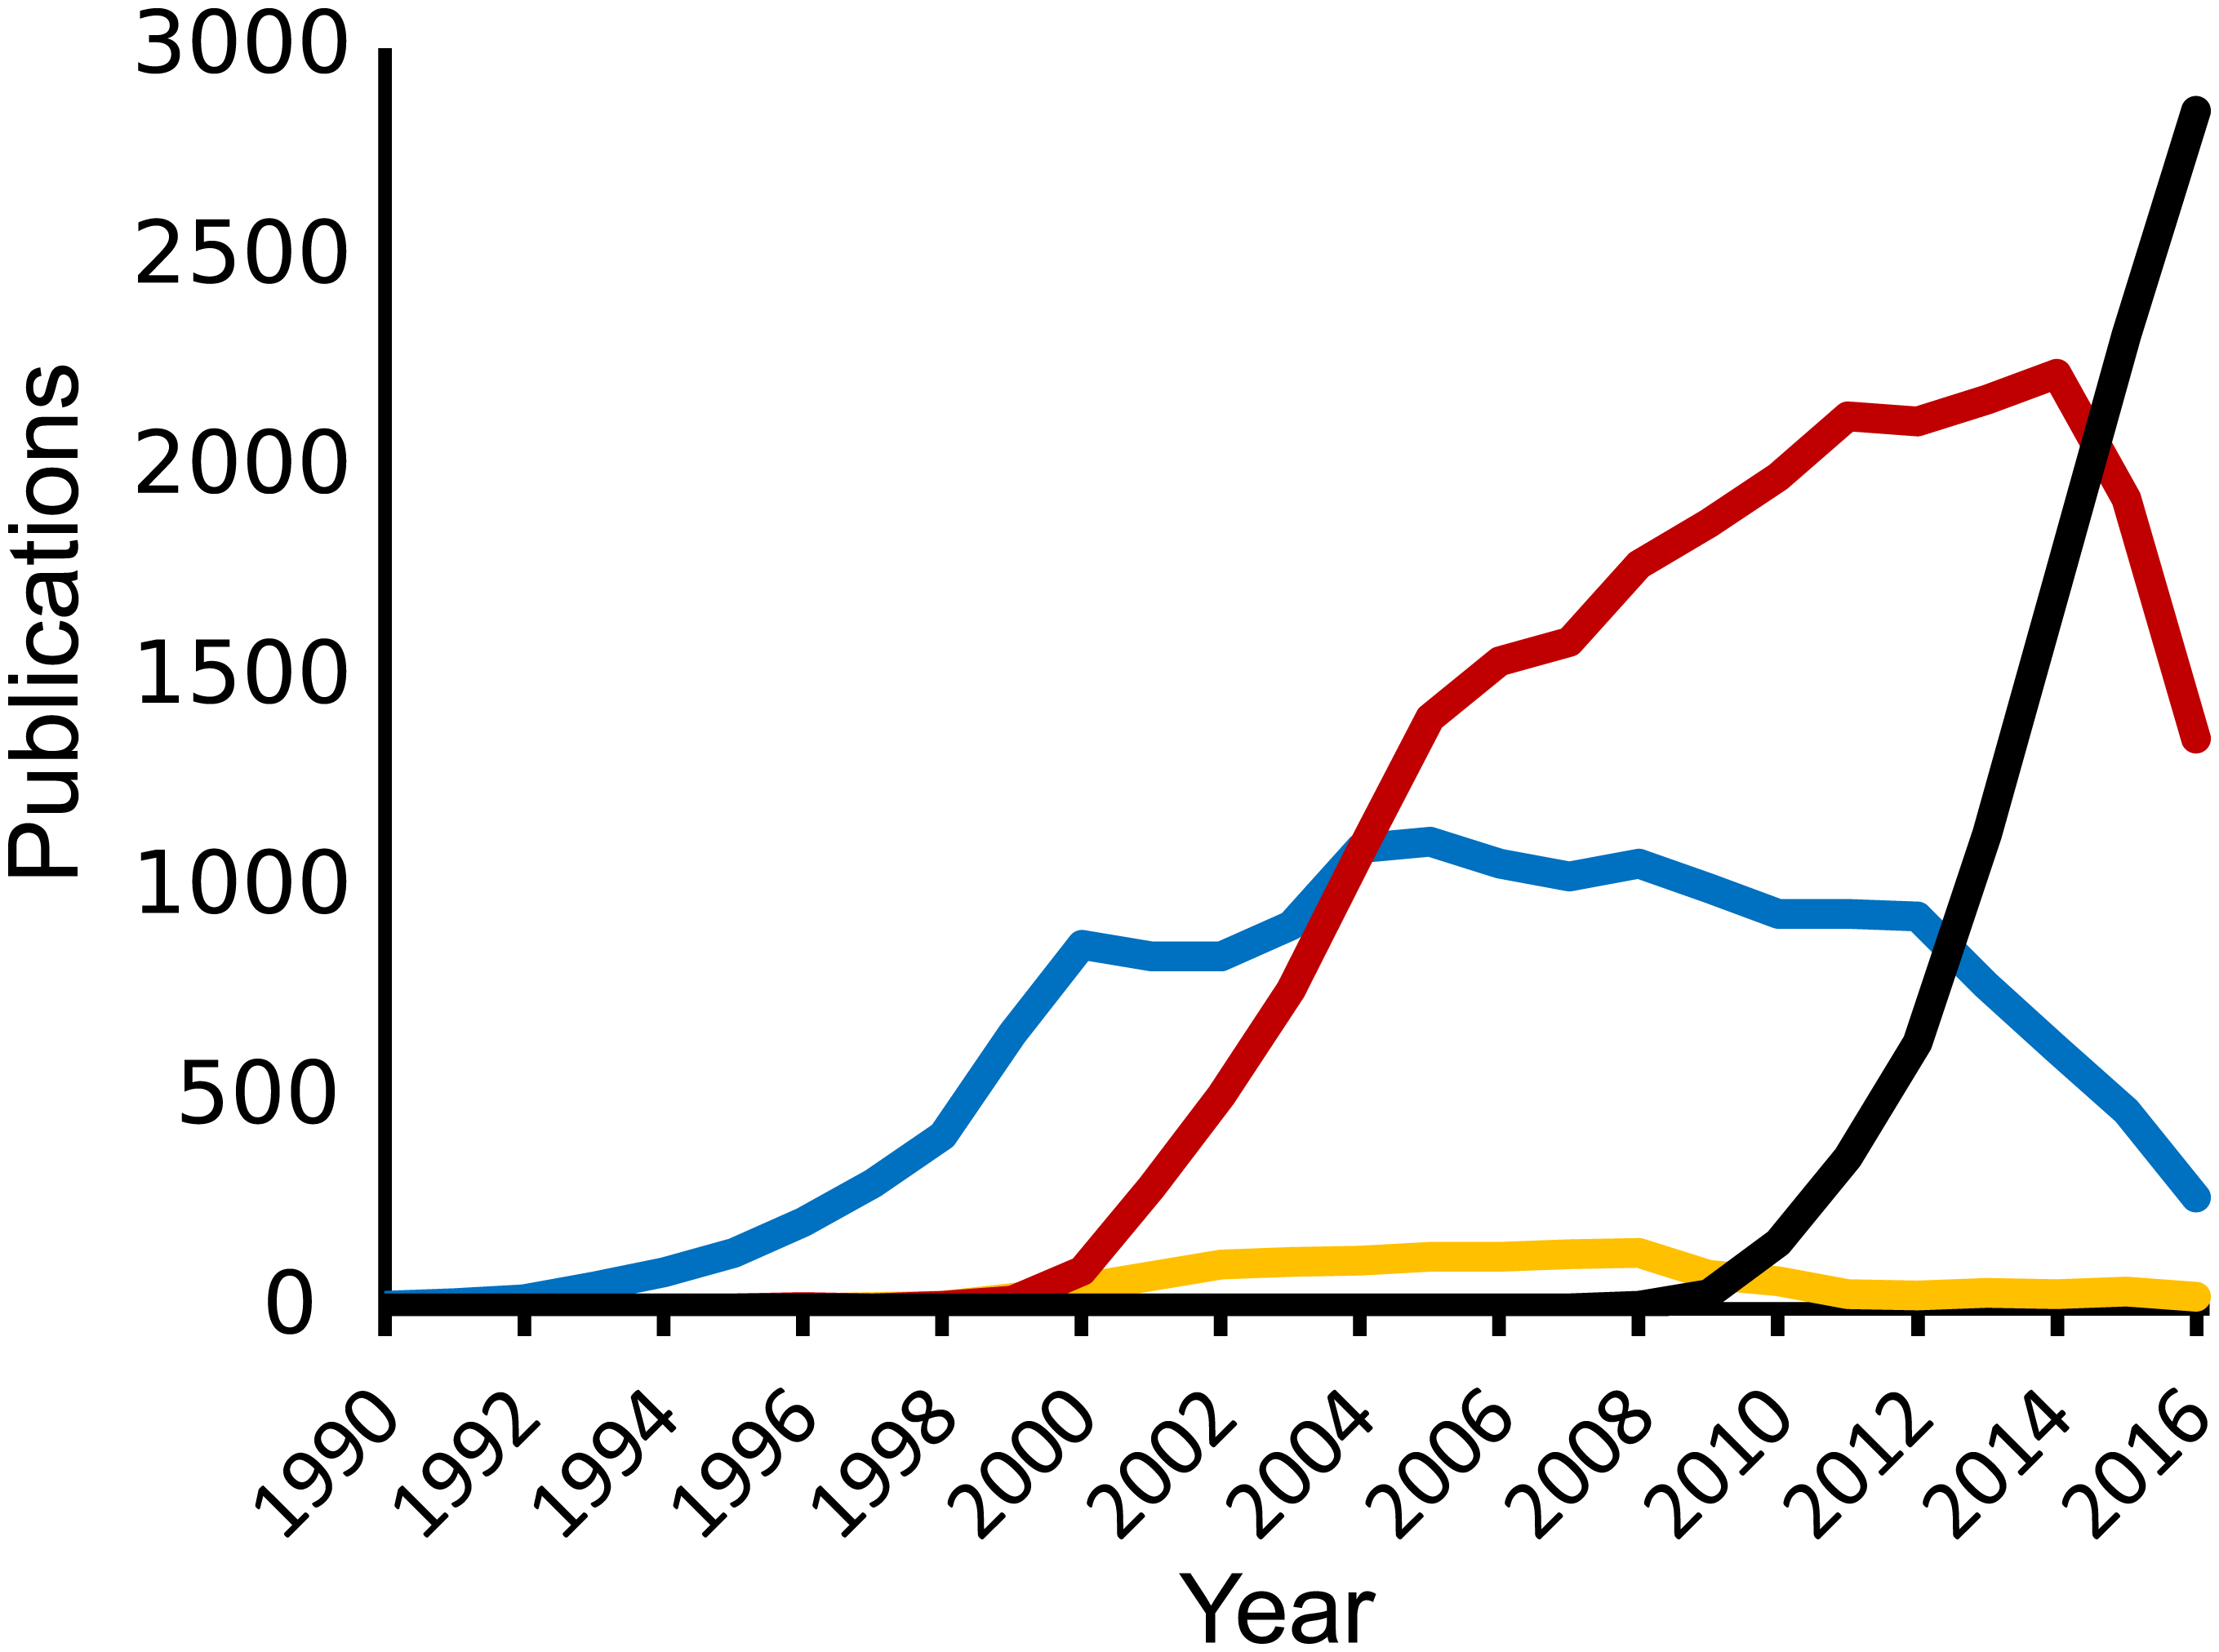
\includegraphics[scale=0.5]{figures/timeTrends.png}		
	~\\
	\textcolor[rgb]{0.1,0.4,0.7}{EST (blue)};
	\textcolor[rgb]{0.85,0.65,0.15}{SAGE / CAGE (yellow)};
	\textcolor[rgb]{0.7,0,0.2}{Microarrays (red)};  
	RNA Seq (black) \footfullcite{2017transcriptomictech}
	\end{center}

\end{frame}

\begin{frame}{Microarrays}

	\begin{itemize}
		\item Microarrays effectively ushered in the modern era of transcriptomics
		\item Purely interested in \textit{relative abundances}
		\item Could measure expression levels for 1000’s of genes simultaneously, for \textit{the first time}		
		\item Were essentially glass slides with probes affixed to them
	\end{itemize}

\end{frame}

\begin{frame}{Microarrays}

	\begin{itemize}
		\item Once again depends on reverse transcriptase for mRNA $\rightarrow$ cDNA
		\item \textbf{No reliance on Sanger Sequencing}
		\item Used probes (like a Northern blot) but the \textbf{cDNA is labelled and the probes are spatially fixed}
		\begin{itemize}
			\item Probes must be designed beforehand
			\item Probes are fixed to the array in \textit{known locations}		
		\end{itemize}
	\end{itemize}
	
\end{frame}

\begin{frame}{Microarrays}

	\begin{enumerate}

		\item Fluorescent labelling during mRNA conversion to cDNA
		\item Complimentary probes bind target sequences (hybridisation)
		\item Fluorescence detection at each probe
	
	\end{enumerate}

	\begin{center}
	\textbf{Fluorescence Intensity $\propto$ mRNA abundance	}
	\end{center}

\end{frame}

\begin{frame}{Microarrays}

	\begin{center}
		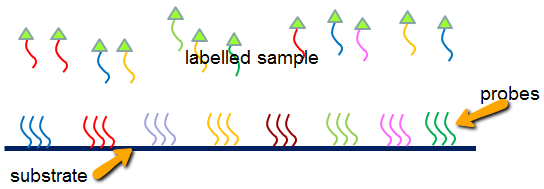
\includegraphics[scale=0.5]{figures/microarray_diagram.png} 
		~\\[8mm]
		\pause
		Highly abundant targets will yield more signal after hybridisation\\[2mm]
		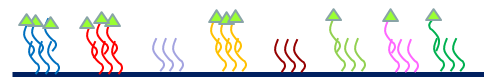
\includegraphics[scale=0.5]{figures/microarray_diagram_02.png} 
	\end{center}
	
	\blfootnote{Source: \url{https://dev.stat.vmhost.psu.edu/stat555/book/export/html/635}}	

\end{frame}

\begin{frame}{Microarrays}

	\begin{center}
	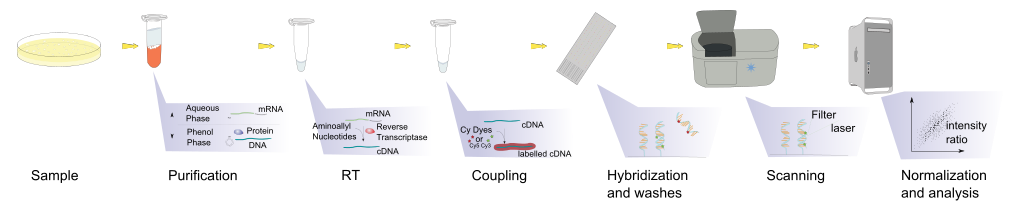
\includegraphics[scale=0.4]{figures/Microarrayhorizontal.png} 
	\end{center}
	
	\blfootnote{Source: \url{https://commons.wikimedia.org/wiki/File:Microarray\_exp\_horizontal.svg}}

\end{frame}

\section{Two Colour Microarrays}

\begin{frame}{Two Colour Microarrays}

	\begin{itemize}
		\item Sometimes called ``Low-Density Oligo Microarrays"
		\item Probes with known sequences are at known locations
		\begin{itemize}
			\item Probes were 60-75mer complimentary cDNA
			\item Originally printed in local facilities
		\end{itemize}
		\item Samples are labelled with \textit{either} Cy3 (Green @ 570nm) or Cy5 (Red @ 670nm)
		\item Two samples are hybridised to each array
		\begin{itemize}
			\item Competitive hybridisation
			\item Relative Red/Green intensities were of interest
			\item Gave an estimate of logFC within each array		
		\end{itemize}
	\end{itemize}

\end{frame}

\begin{frame}{Two Colour Microarrays}

	\begin{center}
	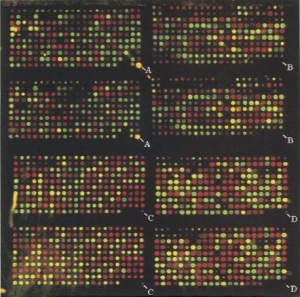
\includegraphics[scale=0.5]{figures/2colour.jpg} 
	~\\
	A section of a two colour array\footfullcite{Shalon01071996}
	\end{center}

\end{frame}

\begin{frame}{Two Colour Microarrays}

	\begin{itemize}
		\item Probes are ``printed" to the array
		\begin{itemize}
			\item Print tips can get clogged and be uneven
		\end{itemize}
		\item Able to be customised for your own experiment
		\begin{itemize}
			\item A mapping file for probe location to target sequence is required
		\end{itemize}
		\item Both colours were scanned separately
		\begin{itemize}
			\item One scan detects red only, the next detects green only
			\item Each individual scan would have to be aligned spatially with the other
		\end{itemize}
		
	\end{itemize}

\end{frame}

\begin{frame}{Two Colour Microarrays}

	\begin{itemize}
		\item Spots were detected using astronomical software
		\begin{itemize}
			\item Sizes were variable / irregular
		\end{itemize}
		\item Detection of true signal above background (DABG)
		\begin{itemize}		
			\item Required ``identified" (foreground) pixels and surrounding (background) pixels
			\item Used surrounding pixels to estimate BG
			\item Assumed BG was additive, e.g. $R = R_{bg} + R_{fg}$
		\end{itemize}
		\item Dye bias was also noted $\implies$ experiments often used dye swaps
		\begin{itemize}
			\item A sample from ``group 1" might be labelled with red on one array, then labelled with green on the next
		\end{itemize}
	\end{itemize}

\end{frame}

\begin{frame}{Two Colour Microarrays}

	\begin{itemize}
		\item All intensities are transformed to the $\log_2$ scale
		\item Dye bias was checked using ``MA Plots"
		\begin{itemize}
			\item $M$ was the \textit{difference in intensity} across both channels
			\item $A$ was the \textit{average intensity} across both channels
		\end{itemize}
	\end{itemize}
	\begin{align*}
		M &= \log_2 R - \log_2 G\\[3mm]
		A &= \frac{\log_2 R + \log_2 G}{2}
	\end{align*}

\end{frame}

\begin{frame}{Two Colour Microarrays}

	\begin{center}
		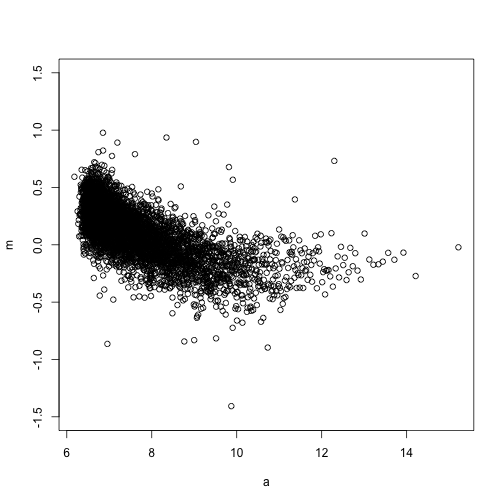
\includegraphics[scale=0.3]{figures/MA_plot.png} 
	\end{center}

\blfootnote{Source: \url{https://genomicsclass.github.io/book/pages/normalization.html}}	


\end{frame}

\begin{frame}{Two Colour Microarrays}

	\begin{center}
		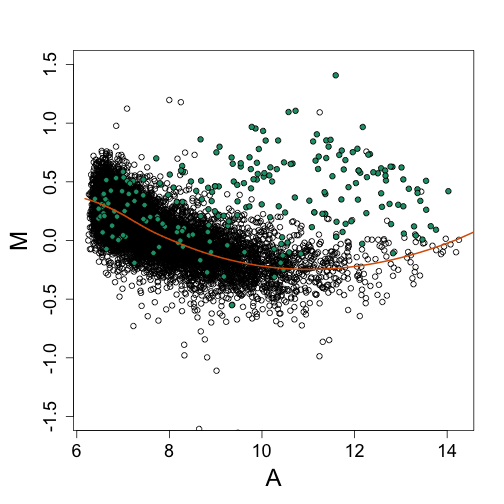
\includegraphics[scale=0.3]{figures/MA_plot_loess.png} 
		~\\
		We can fit a \textbf{loess} curve through the data\\
		(Here, spike-in controls are also highlighted)
	\end{center}

\blfootnote{Source: \url{https://genomicsclass.github.io/book/pages/normalization.html}}	


\end{frame}

\begin{frame}{Two Colour Microarrays}

	\begin{itemize}
		\item \texttt{loess}: Locally estimated scatterplot smoothing
		\begin{itemize}
			\item We use a sliding window and fit a polynomial line
			\item Usually polynomial of order 1 (linear) or 2 (quadratic)
		\end{itemize}
		\item Once we have the loess curve: we subtract it from the data
		\begin{itemize}
			\item Explicitly assumes that the bulk of the difference is bias, i.e. \textit{most genes are not differentially expressed}
			\item No modification to the $A$ values, or any R/G intensities
		\end{itemize}
	\end{itemize}


\end{frame}

\begin{frame}{Two Colour Microarrays}

	\begin{center}
		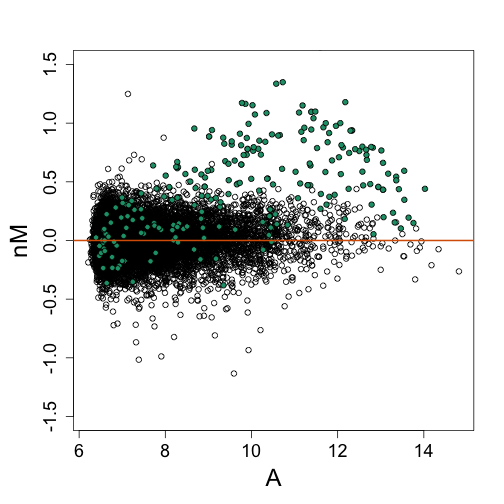
\includegraphics[scale=0.3]{figures/MA_plot_loess_norm.png} 
		~\\
		No more dye bias $\ldots$
	\end{center}

\blfootnote{Source: \url{https://genomicsclass.github.io/book/pages/normalization.html}}	


\end{frame}


\begin{frame}{Two Colour Microarrays}

	\begin{itemize}
		\item We use these normalised $M$ values across arrays to estimate logFC 
		\item Dye-swap complications $\implies$ \textit{Experimental Design}
		\item Robust suite of statistical tools developed from here
		\item The \texttt{R} package \texttt{limma} set the standard
	\end{itemize}

\end{frame}

\section{Single Channel Microarrays}


\begin{frame}{Single Channel Microarrays}

	\begin{itemize}
		\item Affymetrix 3’ Arrays became the dominant technology (until RNA seq)
		\item Probes target the 3’ end of transcripts $\implies$ intact transcripts
		\item Single channel (i.e. single colour) $\implies$ one sample per array
		\item $\sim$1,000,000 $\times$ 25-mer probes
	\end{itemize}
	
	\begin{center}
		\textbf{Fluorescence Intensity $\propto$ mRNA abundance	}
	\end{center}

\end{frame}

\begin{frame}{Single Channel Microarrays}

	\begin{center}
	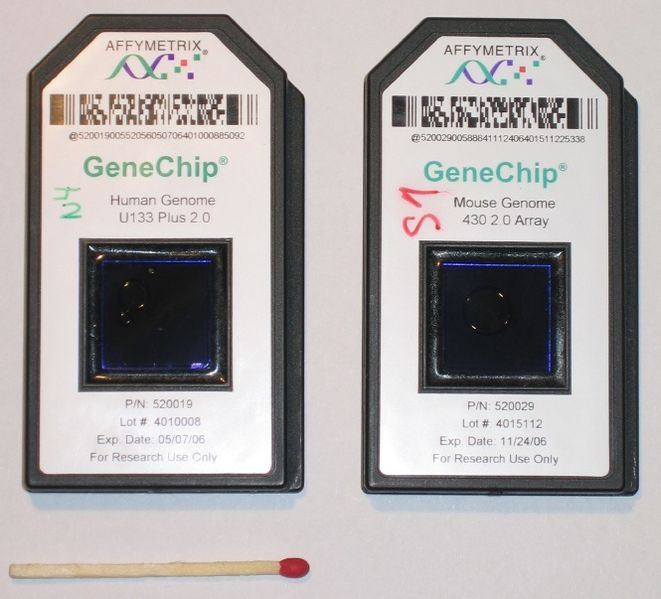
\includegraphics[scale=0.25]{figures/Affymetrix.jpg} 
	\end{center}
	
	\blfootnote{Source: \url{https://commons.wikimedia.org/wiki/File:Affymetrix-microarray.jpg}}

\end{frame}


\begin{frame}{Single Channel Microarrays}

	\begin{itemize}
		\item Manufacture used photolithography
		\item Far greater density of probes than two-colour arrays
		\begin{itemize}
			\item Shorter probes but far more of them
		\end{itemize}
		\item Fixed array designs for each ``model" and organism
		\item Probes designed based on known gene annotations at design-time 
		\item Also need a mapping file from location to probe sequence
	\end{itemize}

\end{frame}

\begin{frame}{Single Channel Microarrays}

	\begin{center}
	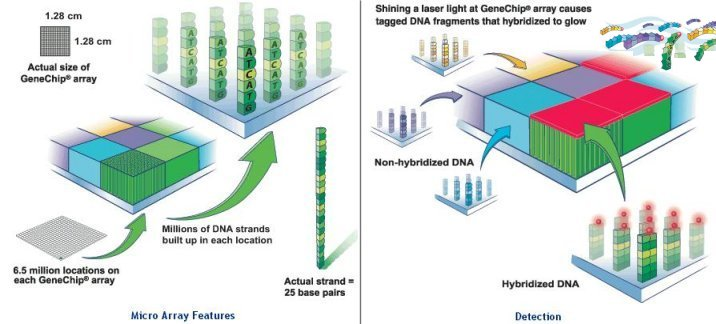
\includegraphics[scale=0.4]{figures/microarrayLayout.jpg} 
	\end{center}
	
	\blfootnote{Source: \url{https://universe-review.ca/R11-16-DNAsequencing.htm}}

\end{frame}

\begin{frame}{3’ Arrays}

	\begin{itemize}
		\item Each 3' exon would be targeted by 11 unique probes
		\begin{itemize}
			\item The set of \textbf{11 probes} would be collected together as a single \textbf{probeset}
		\end{itemize}
		\item Alternate isoforms with different 3' exons could be detected easily as they would have distinct probesets
		\item Need a \textit{Chip Description File} to map probes to array coordinates and probesets
	\end{itemize}


\end{frame}

\begin{frame}{3’ Arrays}

	Key Technical Issues: 

	\begin{enumerate}
		\item Differences between \textbf{arrays}
		\begin{itemize}
			\item Hybridisation artefacts, cDNA/RNA concentration artefacts
		\end{itemize}
		\item Background Correction at the \textbf{probe} level
		\begin{itemize}
			\item 25-mer probes $\implies$ \textit{non-specific binding}
			\item Optical Background
		\end{itemize}
		\item Expression estimates at the \textbf{probeset} level
		\begin{itemize}
			\item Some probes \textit{unresponsive}, other probes \textit{promiscuous}
			\item Do you just \textit{average them}?
		\end{itemize}
	\end{enumerate}
	
\end{frame}

\begin{frame}{Normalisation}

	\begin{center}
		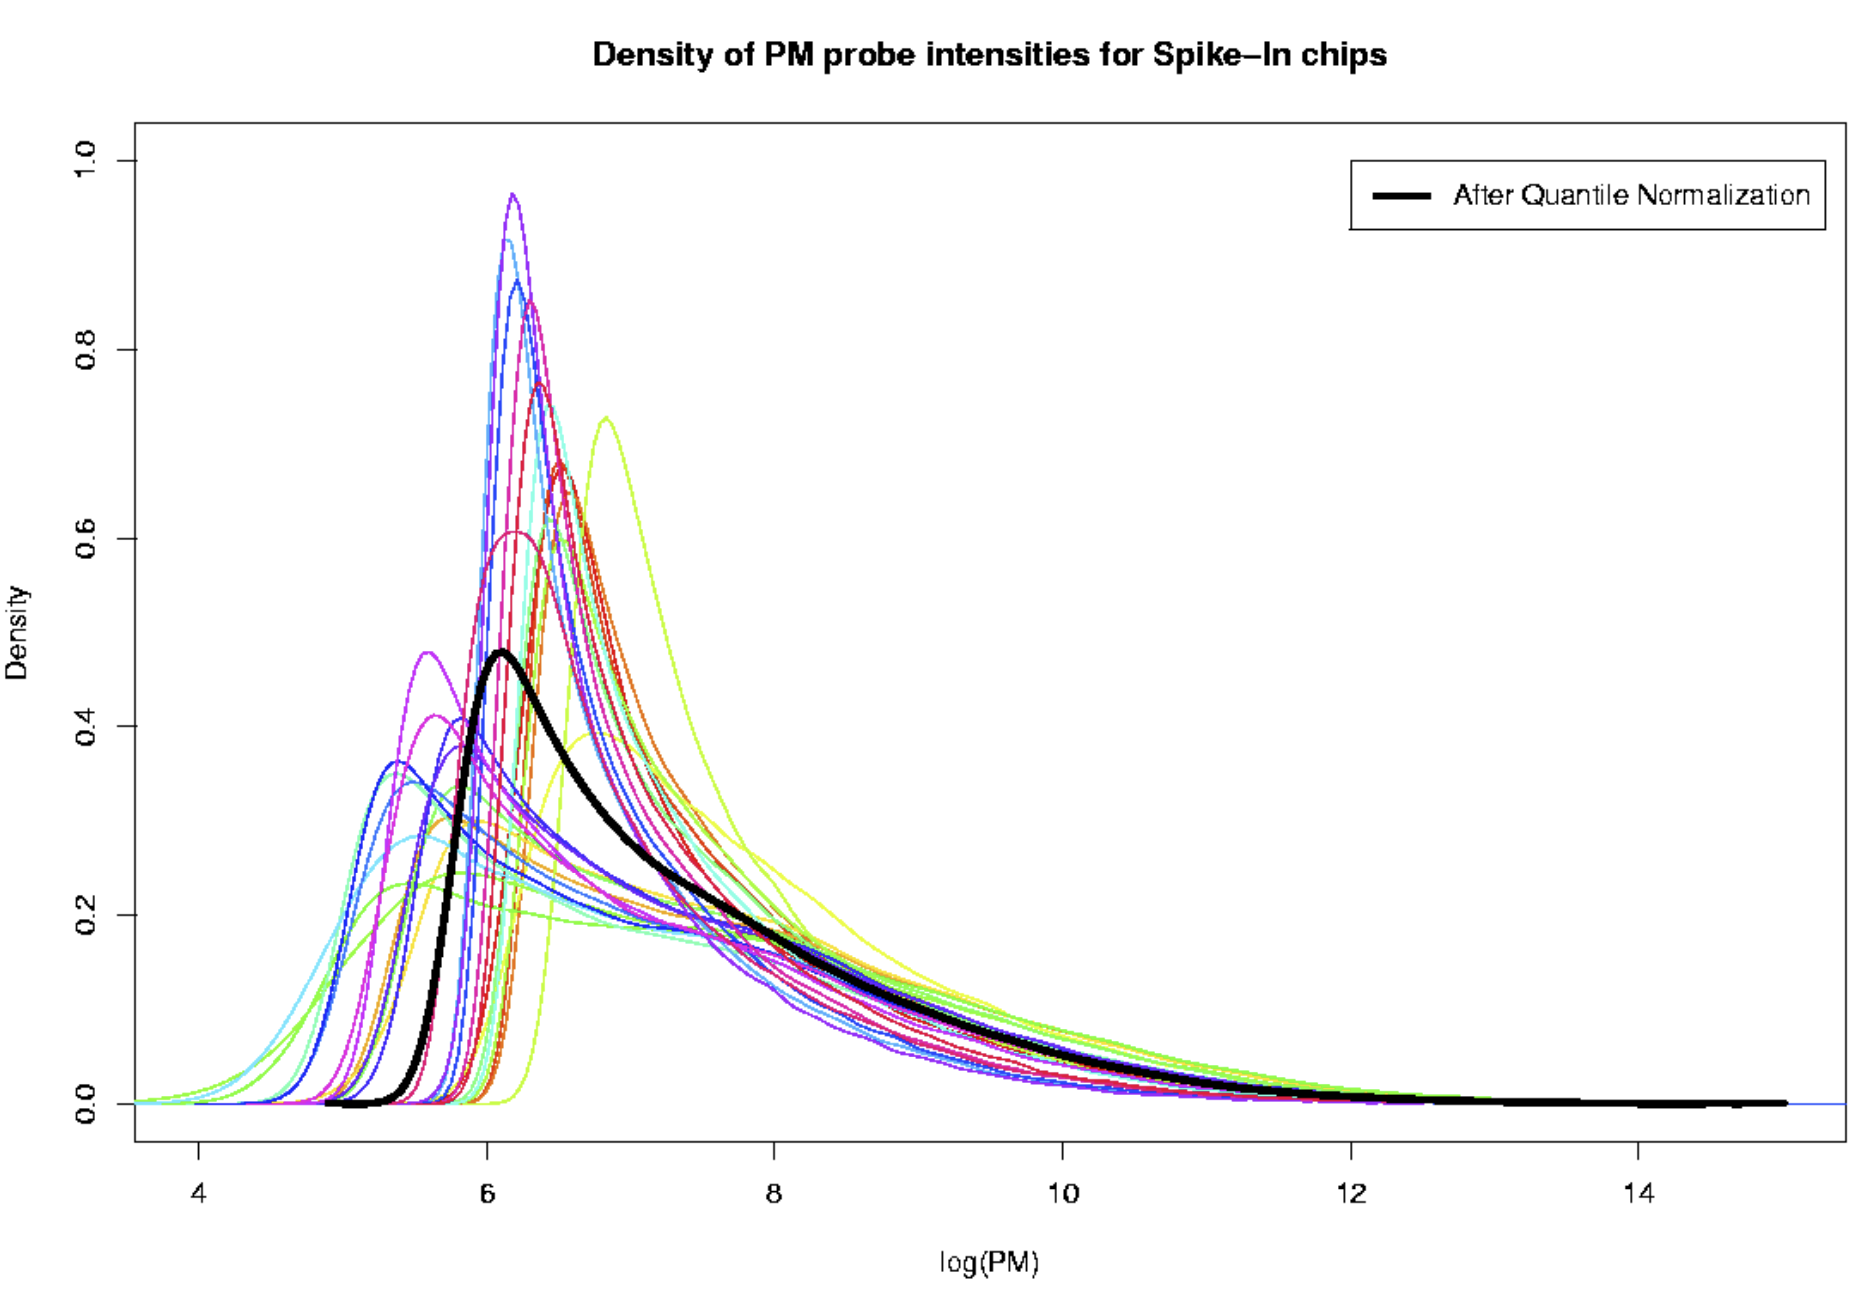
\includegraphics[scale=0.12]{figures/quantileNorm.png} 
	\end{center}

\blfootnote{Taken from \cite{pmid12538238}}	

\end{frame}

\begin{frame}{Quantile Normalisation}

	\begin{enumerate}
		\item Find the probe with the lowest intensity on each array
		\begin{itemize}
			\item This will be from different probesets and unrelated to each other
		\end{itemize}
		\item Find the average intensity across	these probes
		\item Assign this value to each probe
		\item Repeat for the probes with the next lowest intensity until done
		\item All arrays now have the same intensity distribution
	\end{enumerate}
	
	~\\[2mm]	
	Under this approach, \textbf{we are adjusting the raw intensities}

\end{frame}

\begin{frame}{Quantile Normalisation}

	\begin{center}
		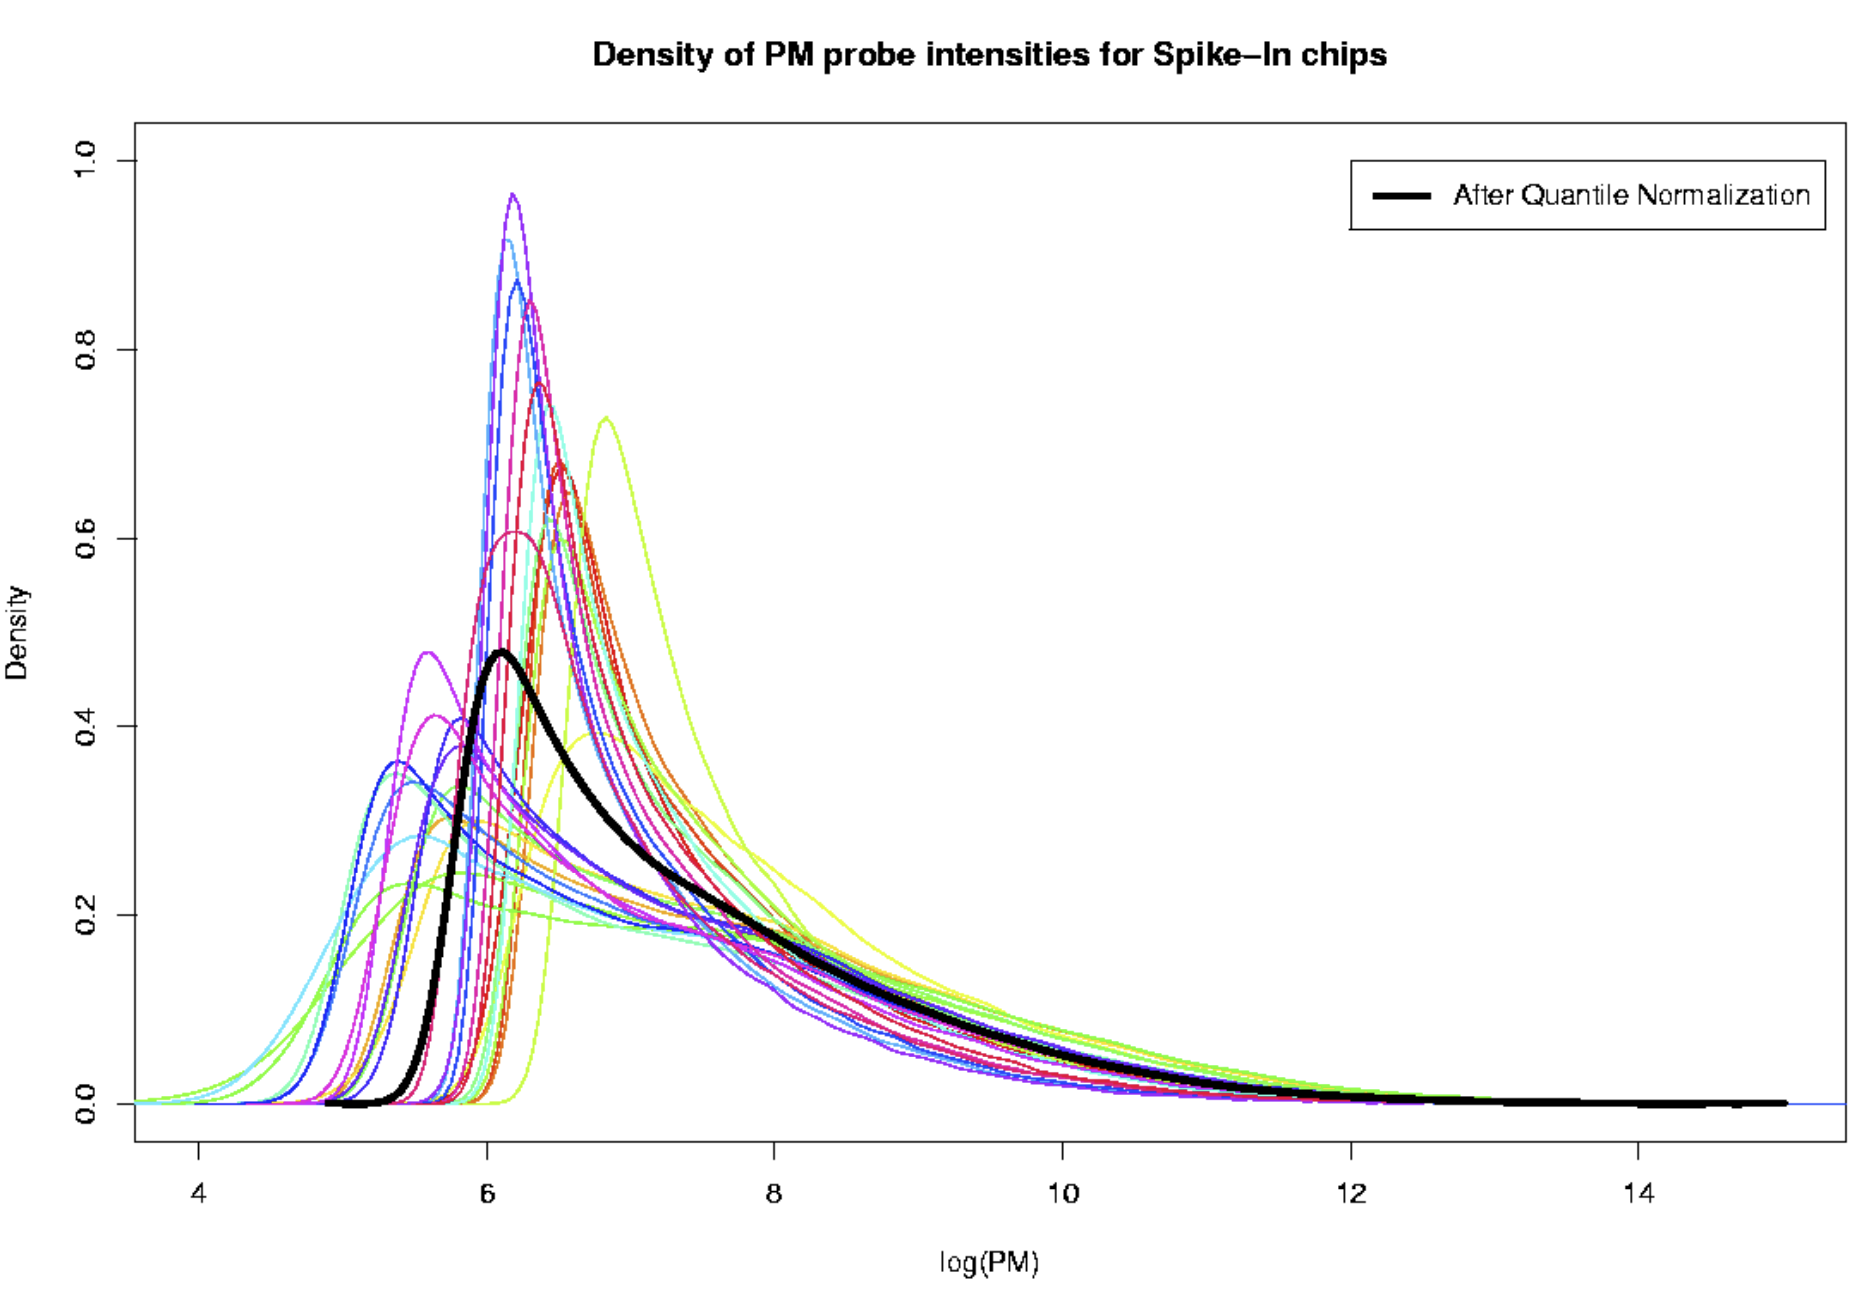
\includegraphics[scale=0.12]{figures/quantileNorm.png} 
	\end{center}

\blfootnote{Taken from \cite{pmid12538238}}	

\end{frame}

\begin{frame}{Quantile Normalisation}

	\begin{center}
		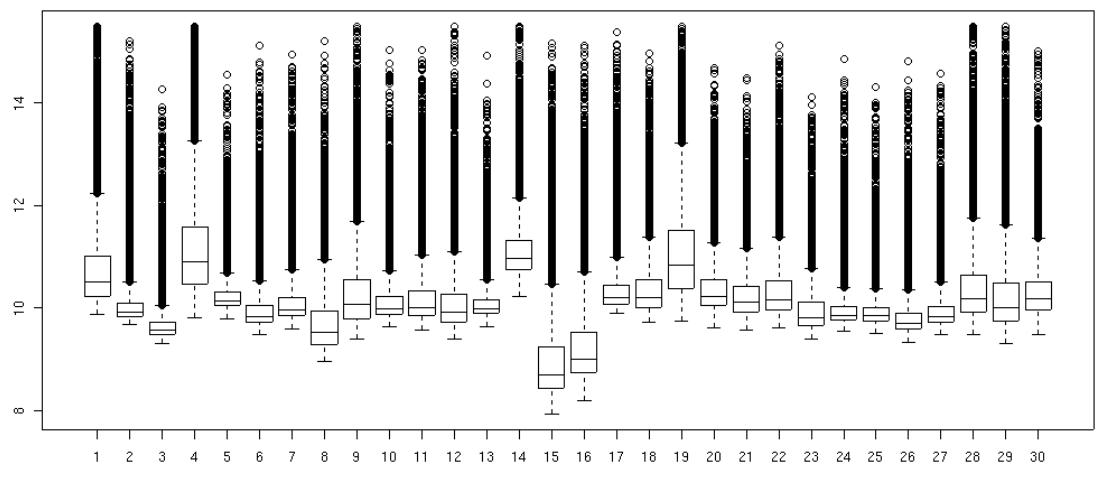
\includegraphics[scale=0.17]{figures/preNorm.png} 
		~\\
		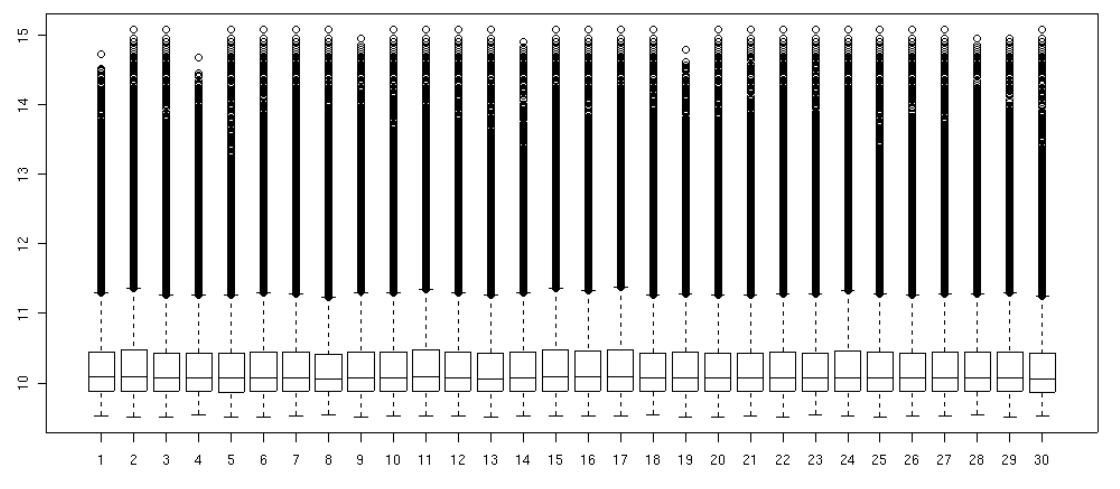
\includegraphics[scale=0.17]{figures/postNorm.png} 
	\end{center}

\blfootnote{Source: Bolstad, Probe Level Quantile Normalization for High Density Oligonucleotide Array Data Unpublished Manuscript, 2001}	

\end{frame}



\begin{frame}{Background Correction}

	\begin{itemize}
		\item Probes targeting 3' exons: Perfect Match (\textit{PM}) probes
		\item Probes with middle base changes: MisMatch (\textit{MM}) probes
		\item \textit{MM} probes were expected to capture similar \textit{NSB} behaviours to paired \textit{PM} probe
		\begin{itemize}
			\item Were often \textbf{brighter} than \textit{PM} probes in pair
		\end{itemize}
		\item Literally \textbf{half} of the array was \textit{MM} probes
	\end{itemize}
	
\end{frame}

\begin{frame}{Background Correction}

For a given \textit{PM/MM} probe pair

	\begin{align*}
		PM &= B + S\\[3mm]
		\text{but}\ldots MM &\neq B
	\end{align*}
	
	\begin{itemize}
		\item How do we estimate $S$?
		\item $S \geq 0$	
	\end{itemize}


\end{frame}

\begin{frame}{Background Correction}

	\begin{itemize}
		\item Found $\hat{S} = E[S|PM]$ using a convolution of normal and exponential distributions (\textit{RMA})
		\item GC content and position in probe also impacted \textit{NSB} $\implies$ \textit{GC-RMA}
		\item No need for the \textit{MM} probe as a pair
		\begin{itemize}
			\item \textit{MM} probes still used in estimation of parameters
		\end{itemize}
	\end{itemize}
	
\end{frame}

\begin{frame}{Background Correction}

	\begin{center}
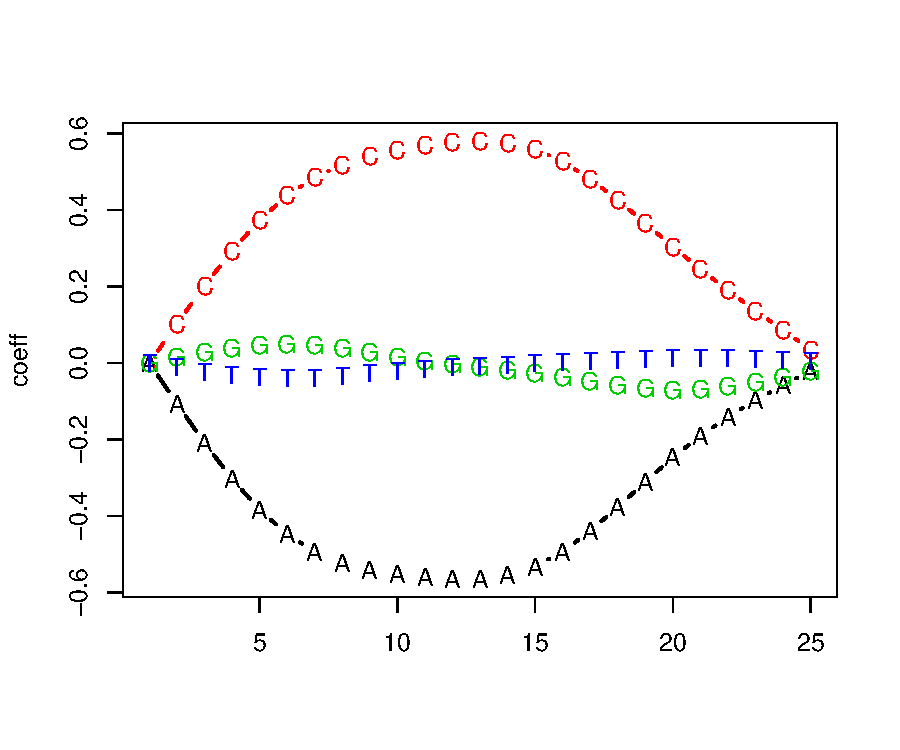
\includegraphics[scale=0.55]{figures/GCRMA_baseprofile.pdf} 
	\end{center}
	
\end{frame}

\begin{frame}{Probeset Summarisation}

	\begin{itemize}
		\item Probes $j = 1, 2, \ldots, 11$ need to be combined (summarised) within a \textbf{probeset}
		\begin{itemize}
			\item This gives the \textbf{gene-level expression estimates} for \textbf{each array}
			\item Poor performing probes were generally poor on all arrays
			\item Promiscuous probes were general similar on all arrays
		\end{itemize}	
		\item Probe-level modelling gave $\mu_i$ for each array $i$
		\begin{itemize}
			\item The model was fit robustly $\implies$ outlier signal is down-weighted
			\item Using $Y_{ij} = \log_2 \hat{S}_{ij}$:
		\end{itemize}
	\end{itemize}

	\begin{align*}
		Y_{ij} = \mu_i + \alpha_j + \varepsilon_{ij}
	\end{align*}
	
	\textbf{Now we have a single, gene-level estimate of expression for each array:} $\hat{\mu}_{i}$
	
\end{frame}

\begin{frame}{Analysis}

	\begin{itemize}
		\item For each gene we take $\hat{\mu}_{i}$ and fit a linear model, conduct a t-test etc
		\item We will deal with the statistics very soon (FUN!)
	\end{itemize}
	
\end{frame}

\begin{frame}{Analysis}
	
The basic process for single channel arrays:

	\begin{enumerate}
		\item Normalise for technical differences
		\item Find probe-level estimates of \textit{true signal}
		\item Obtain gene-level estimates of signal
		\item Statistical Analysis across all genes
	\end{enumerate}

\end{frame}

%\section{Whole Transcript Arrays}
%
%\begin{frame}{Whole Transcript Arrays}
%
%	\begin{itemize}
%		\item The second generation of Affymetrix arrays were Gene/Exon Arrays
%		\item Far greater density of probes ($\sim$5-6 fold)
%		\begin{itemize}
%			\item No \textit{MM/PM} pairs
%			\item Antigenomic and MisMatch probe groups
%		\end{itemize}
%		\item These target the whole transcript (WT), \textbf{NOT} just the 3' end
%		\item How does RNA degradation impact this?
%		\item How does alternate splicing impact this?
%	\end{itemize}
%
%\end{frame}
%
%\begin{frame}{Whole Transcript Arrays}
%
%	\begin{center}
%	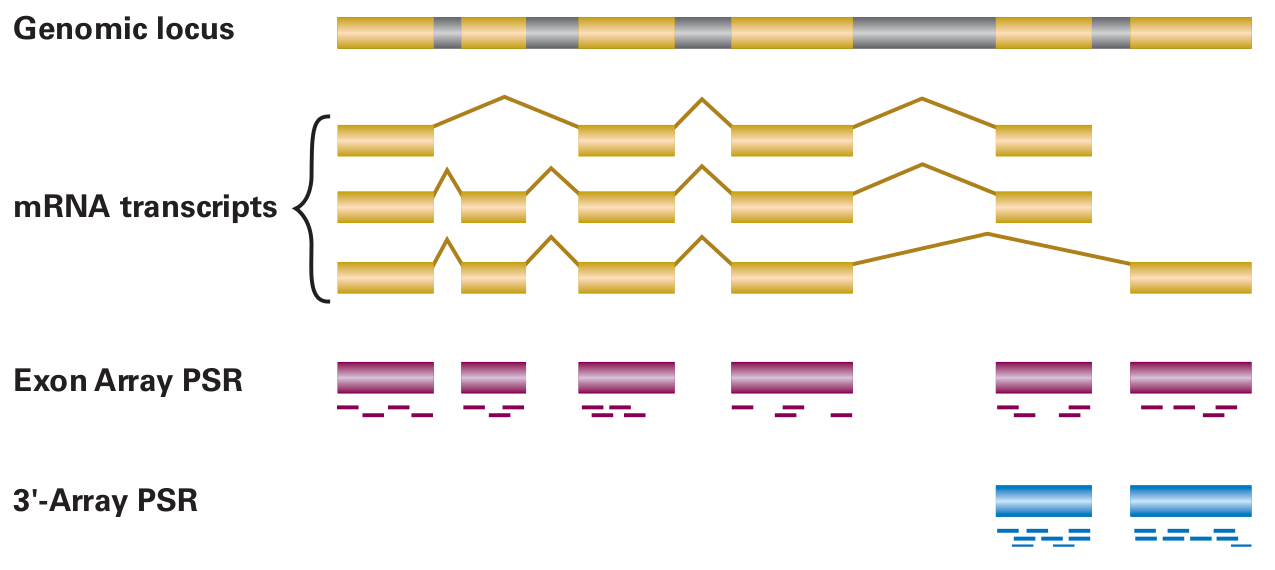
\includegraphics[scale=0.22]{figures/ArrayProbeLayout.png} 
%	\end{center}
%
%\blfootnote{Source: Affymetrix Technical Note}	
%
%\end{frame}
%
%\begin{frame}{Whole Transcript Arrays}
%
%\textbf{RNA Degradation}
%
%	\begin{itemize}
%		\item 3' Arrays had 11 probes targeting the 3' end
%		\item Easily comparable across genes to asses RNA quality
%		\item Not the case for WT Arrays
%	\end{itemize}
%
%\textbf{Alternate Splicing}
%
%	\begin{itemize}
%		\item Identifying the correct transcript remained largely unsolved
%		\item Some exons may be missing
%		\begin{itemize}
%			\item No true signal $implies$ biases expression estimates down
%			\item Can appear as changes in expression, e.g. a short transcript in one condition will yield a lower expression estimate than  a long transcript
%		\end{itemize}
%		
%	\end{itemize}
%
%\end{frame}
%
%\begin{frame}{Whole Transcript Arrays}
%
%	\begin{itemize}
%		\item Before these technical problems were solved RNA Seq ``exploded"
%		\item How do we separate differential expression
%		\begin{itemize}
%			\item i.e. changes in transcriptional activity and regulation
%		\end{itemize}
%		\item from alternate isoform usage
%		\begin{itemize}
%			\item e.g. changes in the dominant isoform, alternate promoter usage
%		\end{itemize}
%		\item Many genes exist in \textit{multiple isoforms in the same tissue}
%	\end{itemize}
%	
%	\textbf{These still remain (somewhat) unsolved in RNA Seq}
%	
%\end{frame}
%
%\begin{frame}{Whole Transcript Arrays}
%
%	\begin{itemize}
%		\item Exon Arrays disappeared very quickly
%		\item Gene Arrays are still in active use (Cheap)
%		\item Both are limited to genes/transcripts defined at time of array design
%		\item Novel transcripts, retained introns etc \textbf{cannot} be detected 
%	\end{itemize}
%
%\end{frame}



\section{Hypothesis Testing}

\begin{frame}{Hypothesis Testing}

In biological research we often ask:

	\begin{center}
	\textbf{“Is something happening?” or “Is nothing happening?”}
	\end{center}

We might be comparing:

	\begin{itemize}
		\item Cell proliferation in response to antibiotics in media
		\item mRNA abundance in two related cell types
		\item Methylation levels across genomic regions
		\item Allele frequencies in two populations
	\end{itemize}

\end{frame}

\begin{frame}{Hypothesis Testing}

	How do we decide if our experimental results are “significant”?

	\begin{itemize}
		\item Is it normal variability?
		\item What would the data look like if our \textit{experiment had no effect?}
		\item What would our data look like if there was \textit{some kind of effect?}
	\end{itemize}
	
	\textbf{Every experiment is considered as a random sample from all possible repeated experiments.}

\end{frame}

\begin{frame}{Sampling}

Most experiments involve measuring something:

	\begin{itemize}
		\item Discrete values e.g. read counts, number of colonies
		\item Continuous values e.g. Ct values, fluorescence intensity
	\end{itemize}

	\textbf{Every experiment is considered as a random sample from all possible repeated experiments.}

\end{frame}

\begin{frame}{Sampling}

	Many data collections can also be considered as experimental datasets
	
	\begin{block}{Example 1}
	In the 1000 Genomes Project a risk allele for T1D has a frequency of $\pi = 0.07$ in European Populations.
	\end{block}
	
	~\\
	\textbf{Does this mean, the allele occurs in exactly 7\% of Europeans?}

\end{frame}

\begin{frame}{Sampling}

	\begin{block}{Example 2}
	In our in vitro experiment, we found that 90\% of HeLa cells were lysed by exposure to our drug.
	\end{block}
	
		\begin{itemize}
			\item Does this mean that exactly 90\% of HeLa cells will always be destroyed?
			\item What does this say about in vivo responses to the drug?
		\end{itemize}

\end{frame}

\begin{frame}{Population Parameters}

	\begin{itemize}
		\item Experimentally-obtained values represent an \textbf{estimate} of the true effect
		\item More formally referred to as \textit{population-level parameters}
		\item Every experiment is considered a \textit{random sample of the complete population}
		\item Repeated experiments would give a \textbf{different} \textit{(but similar)} estimate
	\end{itemize}
	
\pause	
	
	All population parameters are considered to be fixed values, e.g.

	\begin{itemize}
		\item Allele frequency ($\pi$) in a population
		\item The average difference in mRNA levels
	\end{itemize}		


\end{frame}

\begin{frame}{The Null Hypothesis}

 All classical statistical testing involves:
 
 	\begin{enumerate}
			\item a Null Hypothesis ($H_0$) and
			\item an Alternative Hypothesis ($H_A$)
	\end{enumerate}


Why do we do this?
\end{frame}

\begin{frame}{The Null Hypothesis}

	\begin{itemize}
		\item \textit{We define $H_0$ so that we know what the data will look like if there is no effect}
		\item The alternate ($H_A$) includes every other possibility besides $H_0$
	\end{itemize}

An experimental hypothesis may be:\\[3mm]
\begin{block}{Example}
	\begin{align*}
	H_0:\mu=0 \text{ Vs } H_A:\mu \neq 0
	\end{align*} 
	
Where $\mu$ represents the \textit{true average difference in a value }(e.g. mRNA expression levels)

\end{block}




\end{frame}


\end{document}